\documentclass[]{article}
\usepackage{authblk}
\usepackage{hyperref}
\usepackage{graphicx}
\usepackage{float}

\begin{document}
\title{Progressive File Transfer (PFT) Protocol}
\author{
	Jakob Buchgraber
	}

\maketitle
\tableofcontents
\newpage

\begin{abstract}
Lorem ipsum dolor sit amet, consectetur adipiscing elit. Suspendisse tempor ante sit amet felis lobortis, sed vulputate orci ultricies. Nulla sed finibus sapien, ut scelerisque lorem. Maecenas lobortis nisl a ultricies fringilla. Etiam sit amet scelerisque ex, et efficitur libero. Pellentesque et ipsum ac nunc iaculis laoreet et a nunc. Vestibulum dignissim ut nulla interdum tincidunt. Suspendisse eget massa erat. Integer in euismod lorem, quis vehicula ante. Sed sit amet magna ac nisl vehicula semper ac nec orci. Morbi ac mauris est. Pellentesque habitant morbi tristique senectus et netus et malesuada fames ac turpis egestas. Cras mollis vehicula enim bibendum malesuada. Curabitur malesuada ligula at nunc accumsan, non viverra nulla bibendum. Phasellus dapibus tortor at est ultricies iaculis. Sed vitae vulputate nibh.
\end{abstract}


\section{Framing}

The frames are encoded on the wire in a framing format as specified in figure~\ref{framing}.
A PFT frame consists of a fixed 7 octet header and a variable length payload. The first
two octets specify the length of the entire frame, that is of the header and the variable
length payload. The next octet specifies the type of the frame. The last four octets of
the header specify an identifier, which uniquely identifies a connection. The identifier
is a pseudo-random non-zero byte sequence that must be chosen by the server. A server and
client is free to drop any frame with an illegal identifier i.e. zero or unknown. The variable length payload
contains the data of the specific packet type.

\begin{figure}[H]
\centering
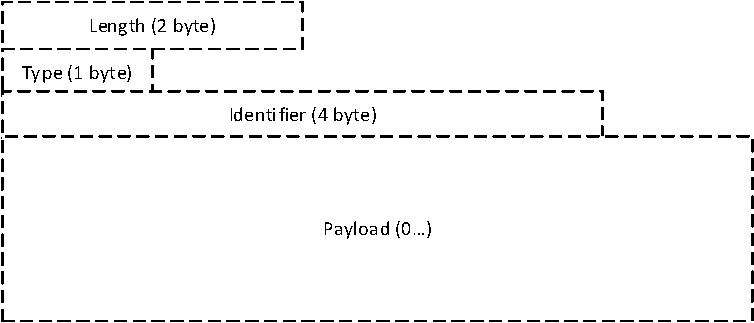
\includegraphics[width=\textwidth]{frames/framing.pdf}
\caption{Framing}
\label{framing}
\end{figure}

\section{Frame Types}


\begin{figure}[H]
\centering
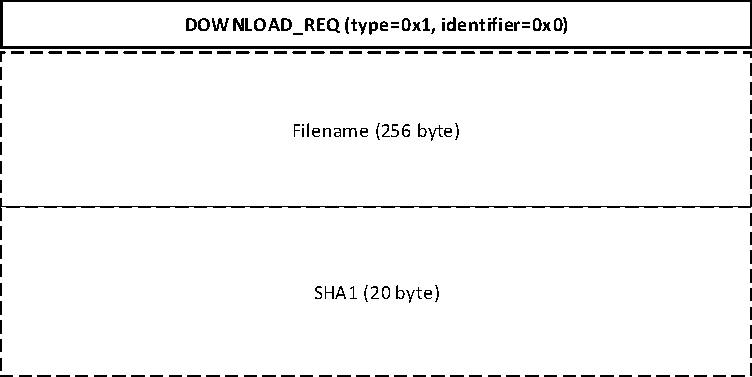
\includegraphics[width=\textwidth]{frames/download-req.pdf}
\caption{DOWNLOAD\_REQ}
\label{DOWNLOAD-REQ}
\end{figure}

\begin{figure}[H]
\centering
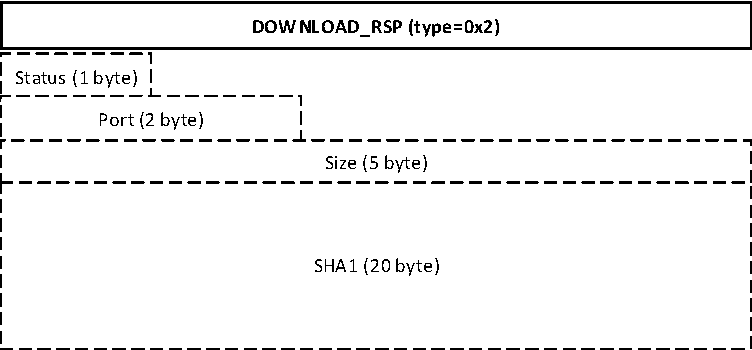
\includegraphics[width=\textwidth]{frames/download-rsp.pdf}
\caption{DOWNLOAD\_RSP}
\label{DOWNLOAD-RSP}
\end{figure}

\begin{figure}[H]
\centering
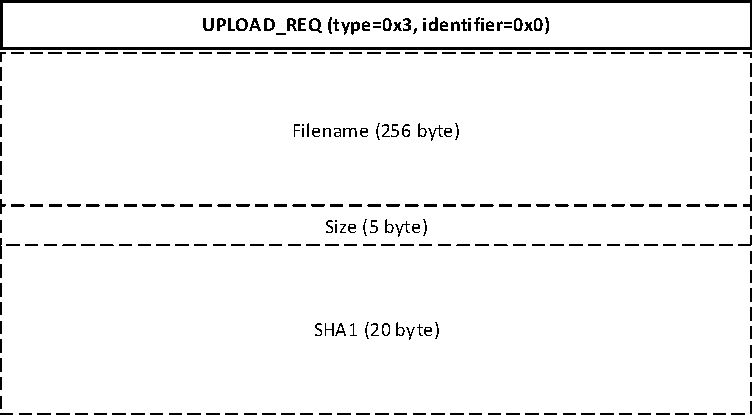
\includegraphics[width=\textwidth]{frames/upload-req.pdf}
\caption{UPLOAD\_REQ}
\label{UPLOAD-REQ}
\end{figure}

\begin{figure}[H]
\centering
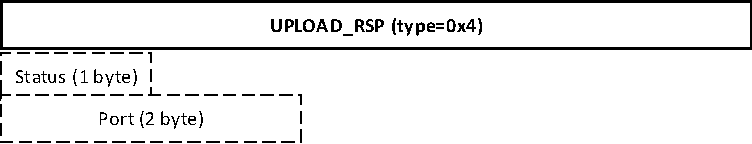
\includegraphics[width=\textwidth]{frames/upload-rsp.pdf}
\caption{UPLOAD\_RSP}
\label{UPLOAD-RSP}
\end{figure}

\begin{figure}[H]
\centering
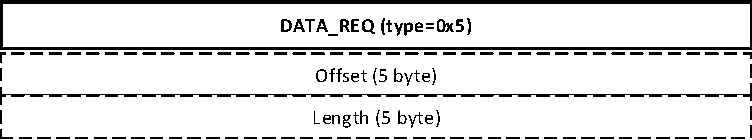
\includegraphics[width=\textwidth]{frames/data-req.pdf}
\caption{DATA\_REQ}
\label{DATA-REQ}
\end{figure}

\begin{figure}[H]
\centering
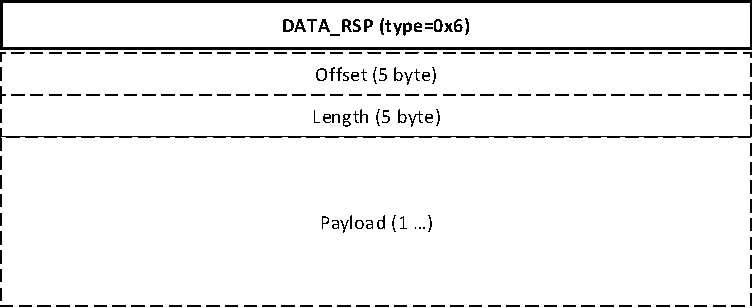
\includegraphics[width=\textwidth]{frames/data-rsp.pdf}
\caption{DATA\_RSP}
\label{DATA-RSP}
\end{figure}

\begin{figure}[H]
\centering
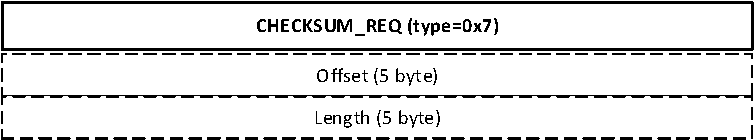
\includegraphics[width=\textwidth]{frames/checksum-req.pdf}
\caption{CHECKSUM\_REQ}
\label{CHECKSUM-REQ}
\end{figure}

\begin{figure}[H]
\centering
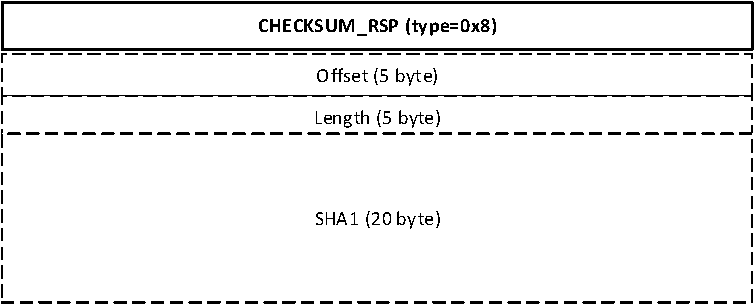
\includegraphics[width=\textwidth]{frames/checksum-rsp.pdf}
\caption{CHECKSUM\_RSP}
\label{CHECKSUM-RSP}
\end{figure}

\begin{figure}[H]
\centering
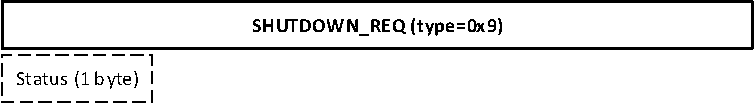
\includegraphics[width=\textwidth]{frames/shutdown-req.pdf}
\caption{SHUTDOWN\_REQ}
\label{SHUTDOWN-REQ}
\end{figure}

\end{document}
